Fernando construye escaleras de ladrillos de la siguiente forma:
\begin{center}
	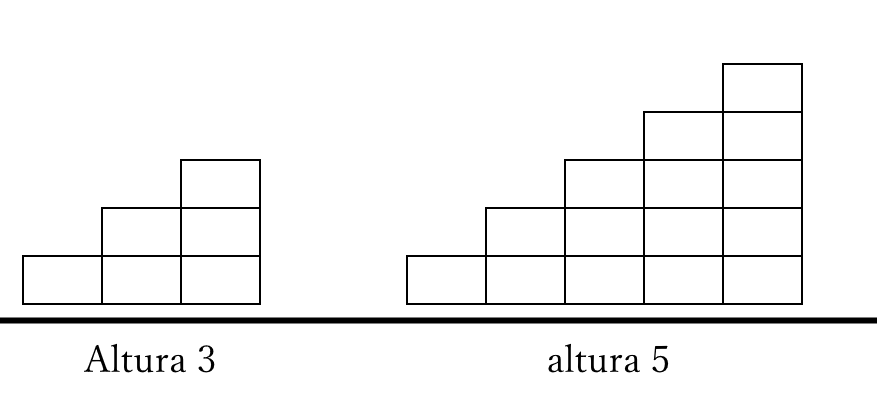
\includegraphics[scale=0.25]{escaleras}
\end{center}

El otro día, Fernando obtuvo \(K\) ladrillos, ahora se pregunta ¿Qué tan alto que puede construir una escalera? Dado \(K\), responde su pregunta.

\begin{plimits}
	\item \(1\leq K \leq 10^9\)
\end{plimits}

\subsubsection{Casos ejemplo}
\begin{casebox2}
	\scase{12}{4}
	\scase{8}{3}
	\scase{20}{5}
\end{casebox2}

Enlace: [TODO]